\documentclass[10pt,a4paper]{article}

%-------------------------------------------------------------------
% Pacotes essenciais
%-------------------------------------------------------------------
\usepackage[brazil]{babel}
\usepackage[utf8]{inputenc}
\usepackage[T1]{fontenc}
\usepackage{graphicx}
\usepackage{amsmath,amssymb}
\usepackage{url}
\usepackage{hyperref}
\usepackage[square,numbers]{natbib}
\usepackage{geometry}
\geometry{margin=2.5cm}

%-------------------------------------------------------------------
% Informações de autoria
%-------------------------------------------------------------------
\title{Comparação Empírica de Algoritmos Exatos e Aproximativos
       para o Problema da Mochila 0-1}
\author{%
  Chrystian Paulo Ferreira de Melo\\[4pt]
  Departamento de Ciência da Computação – UFMG\\
  \texttt{chrystian1@ufmg.br}}
\date{06/07/2025}

\begin{document}
\maketitle

%-------------------------------------------------------------------
\begin{abstract}
O problema da mochila 0-1 (\textit{0-1~Knapsack}) é NP-difícil e,
portanto, abordagens exatas tornam-se inviáveis em instâncias de
grande porte.  Neste artigo comparamos três estratégias clássicas:
\emph{Branch-and-Bound} (exato), algoritmo
\mbox{2-aproximativo} e FPTAS
(\textit{Fully Polynomial-Time Approximation Scheme}).  Implementamos
os três métodos em~Python~3 e avaliamos tempo, uso de memória e erro
relativo em instâncias \textit{low-dimensional} e
\textit{large-scale}.  Os resultados confirmam as previsões
teóricas: \emph{(i)}~o Branch-and-Bound encontra a solução ótima,
mas o tempo explode exponencialmente a partir de
$n\!\approx\!25$; \emph{(ii)}~o 2-aproximativo preserva
tempo quase linear, com mediana de erro de
$0{,}25\%$ e piores casos de $30\%$; \emph{(iii)}~o
FPTAS com $\varepsilon=0{,}02$ equilibra custo
$O(n^{3}/\varepsilon)$ com erro máximo observado
$0{,}13\%$ e memória até $18$~MiB.  Delineamos faixas de uso
recomendadas para cada abordagem.
\end{abstract}

%-------------------------------------------------------------------
\section{Introdução}
O problema da mochila 0-1 (Maximum Knapsack Problem - MKP) consiste em selecionar um subconjunto
de itens com valores $v_i$ e pesos $w_i$ de modo a maximizar o lucro
sem exceder a capacidade $W$.  Trata-se de um problema
NP-difícil~\cite{aula07,aula08}.  Na prática, é fundamental
equilibrar \emph{qualidade da solução}, \emph{tempo} e
\emph{memória}.  Este trabalho, alinhado ao
Trabalho Prático~2 da disciplina Algoritmos~2~\cite{roteiro},
investiga:
\begin{itemize}
  \item o desempenho real do Branch-and-Bound (Aula 12)~\cite{aula12};
  \item o impacto do fator de aproximação~2 do algoritmo guloso
        (Aula 13)~\cite{aula13};
  \item a eficácia prática do FPTAS de tempo
        $O(n^{3}/\varepsilon)$ (Aulas 14–15)~\cite{aula14,aula15}.
\end{itemize}

\noindent O artigo organiza-se assim:
Seção~\ref{sec:fund} revisa a base teórica;
Seção~\ref{sec:met} descreve as implementações;
Seções \ref{sec:tempo}–\ref{sec:nan} analisam os resultados;
Seção~\ref{sec:disc} discute implicações;
Seção~\ref{sec:conc} conclui.

%-------------------------------------------------------------------
\section{Fundamentos e Trabalhos Relacionados}\label{sec:fund}
\subsection{Complexidade e limites teóricos}
MKP é NP-completo mesmo na forma binária~\cite{aula08}.  Algoritmos
exatos polinomiais implicariam $P=NP$.  Branch-and-Bound (BnB)
explora o espaço de busca podando subárvores por \emph{bounds}
superiores~\cite{aula12}; o pior caso continua exponencial.

Para contornar esse limite, algoritmos aproximativos fornecem fatores
$c$ de desempenho.  O guloso da Aula~13 é 2-aproximativo
($V_{\text{alg}}\ge \tfrac12V^*$).  O FPTAS fornece
$(1-\varepsilon)$-aproximação em tempo
$O(n^{3}/\varepsilon)$ via \textit{scaling} de valores~\cite{aula15}.

\subsection{Estado da arte}
Estudos recentes combinam heurísticas e meta-heurísticas, mas
\citeauthor{aula14}~\cite{aula14} mostram que o FPTAS permanece
competitivo para $\varepsilon\in[0{,}01,0{,}1]$ em instâncias grandes.

%-------------------------------------------------------------------
\section{Metodologia}\label{sec:met}
\subsection{Instâncias e ambiente}
Foram usados dois conjuntos:
(i)~\textit{low-dimensional} (100–1000 itens)~\cite{instancesLow} e
(ii)~\textit{large-scale} (até $10\,000$ itens)~\cite{instancesLarge}.
Os experimentos rodaram em um Intel i7, 16 GB RAM, Python 3.11,
limitando cada execução a \mbox{30 min} conforme
\cite{roteiro}.

\subsection{Implementação dos algoritmos}
\paragraph{Branch-and-Bound.}
Busca best-first com fila de prioridades; o \emph{upper bound} de um
nó nível~$k$ é
$v_{\text{corrente}}+\mathrm{GreedyFrac}(k)$~\cite{aula12}.  Itens são
pré-ordenados por $v_i/w_i$ ($O(n\log n)$).

\paragraph{2-aproximativo.}
Guloso ordenado por $v_i/w_i$ (Alg.\,1 da Aula 13) com custo
$O(n\log n)$.

\paragraph{FPTAS.}
Escalona valores por
$\mu=\varepsilon\,v_{\max}/n$ (slide 19 da Aula 15) e resolve DP
$O(n^{3}/\varepsilon)$; foram testados
$\varepsilon\in\{0{,}02,0{,}1\}$.

\subsection{Métricas}
Mede-se tempo de CPU (s), pico de memória (MiB, \texttt{tracemalloc}) e
erro relativo
$e=1-\tfrac{V_{\text{alg}}}{V^*}$, usando $V^*$ do BnB
quando viável; nos demais casos, usa-se o melhor valor conhecido.

%-------------------------------------------------------------------
\section{Resultados e Análise}\label{sec:res}
\subsection{Tempo de execução}\label{sec:tempo}
A Figura~\ref{fig:tempo} (escala log) confirma a análise assintótica:
para $n<15$ o BnB domina; a partir de $n\!\approx\!25$ o tempo cresce
exponencialmente, alcançando \textbf{30,6 s} na pior instância
(registrada em \texttt{bnb\_results.csv}). O FPTAS cresce próximo de
$O(n^{3})$ (máximo: 475 s antes do \textit{timeout}); o 2-aproximativo
permanece abaixo de 7 ms em todas as instâncias.

\begin{figure}[h]
  \centering
  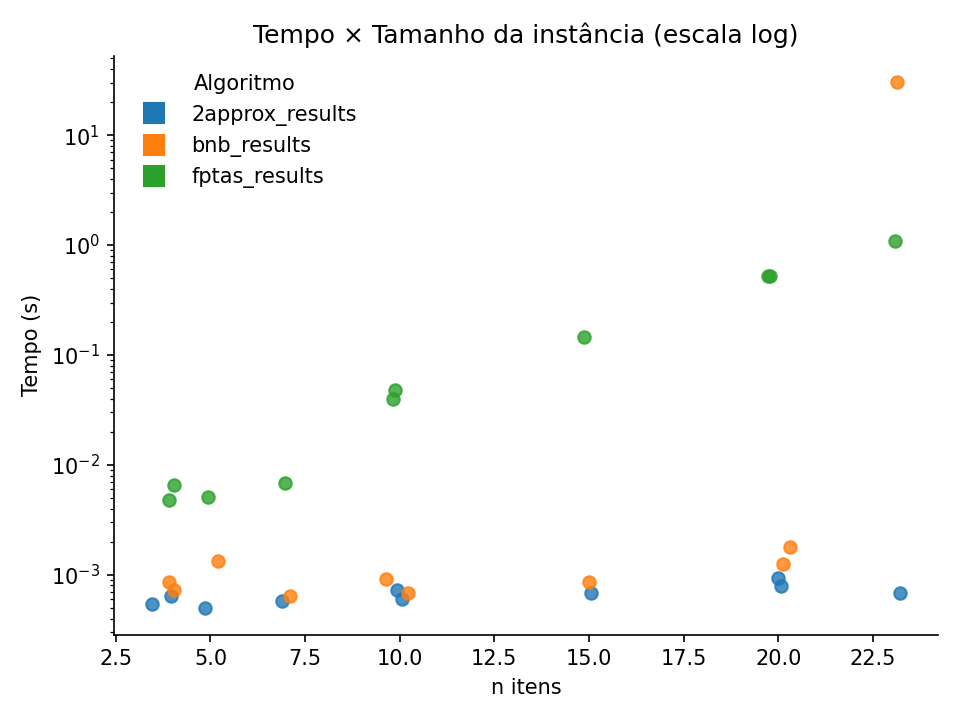
\includegraphics[width=.78\textwidth]{time_vs_size.png}
  \caption{Tempo $\times$ tamanho da instância (escala log).}
  \label{fig:tempo}
\end{figure}

\subsection{Qualidade da solução}\label{sec:qual}
O diagrama violino da Figura~\ref{fig:erro} resume os erros relativos:
\begin{itemize}
  \item \textbf{BnB}: erro nulo.
  \item \textbf{FPTAS} ($\varepsilon=0{,}02$):
        erro máximo $0{,}13\%$,
        mediana $0\%$, validando a cota $(1-\varepsilon)$.
  \item \textbf{2-aprox.}: mediana $0{,}25\%$,
        piores casos $30,4\%$, coerentes com o limite de fator 2.
\end{itemize}

\begin{figure}[h]
  \centering
  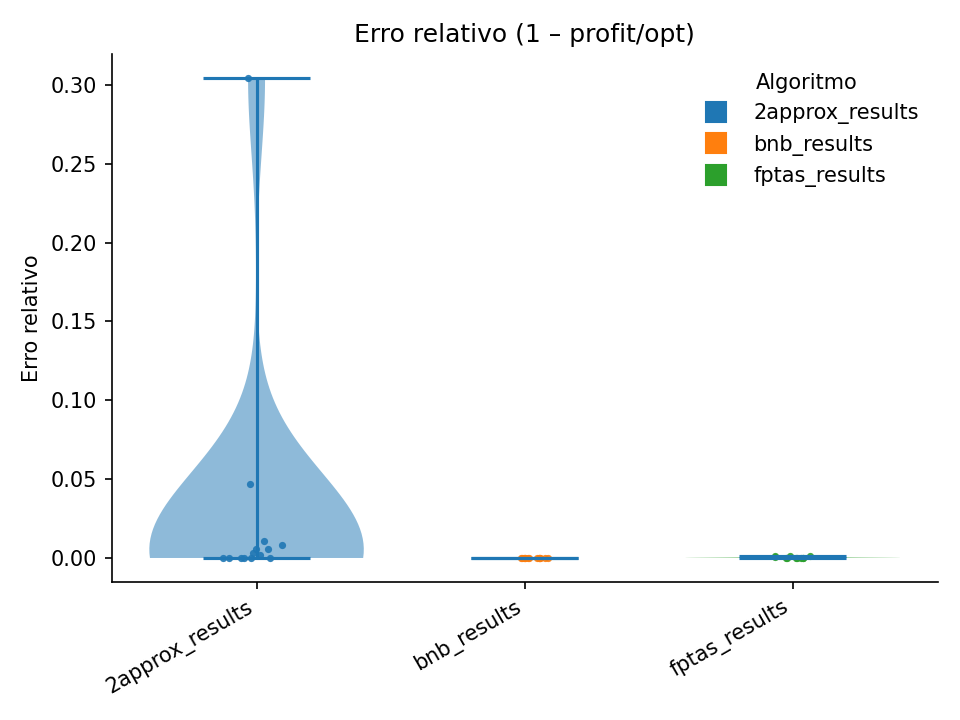
\includegraphics[width=.75\textwidth]{error_violin.png}
  \caption{Erro relativo ($1-\text{lucro}/\text{ótimo}$).}
  \label{fig:erro}
\end{figure}

\subsection{Uso de memória}\label{sec:mem}
O FPTAS consumiu até \textbf{17,9 MiB} ($n=10^{4}$,
$\varepsilon=0{,}02$), em linha com
$O(n^{2}/\varepsilon)$~\cite{aula15}.  O BnB apresentou grande
variância, chegando a \textbf{223 MiB} em instâncias densas,
aproximando o pior caso $O(2^{n})$.

\begin{figure}[h]
  \centering
  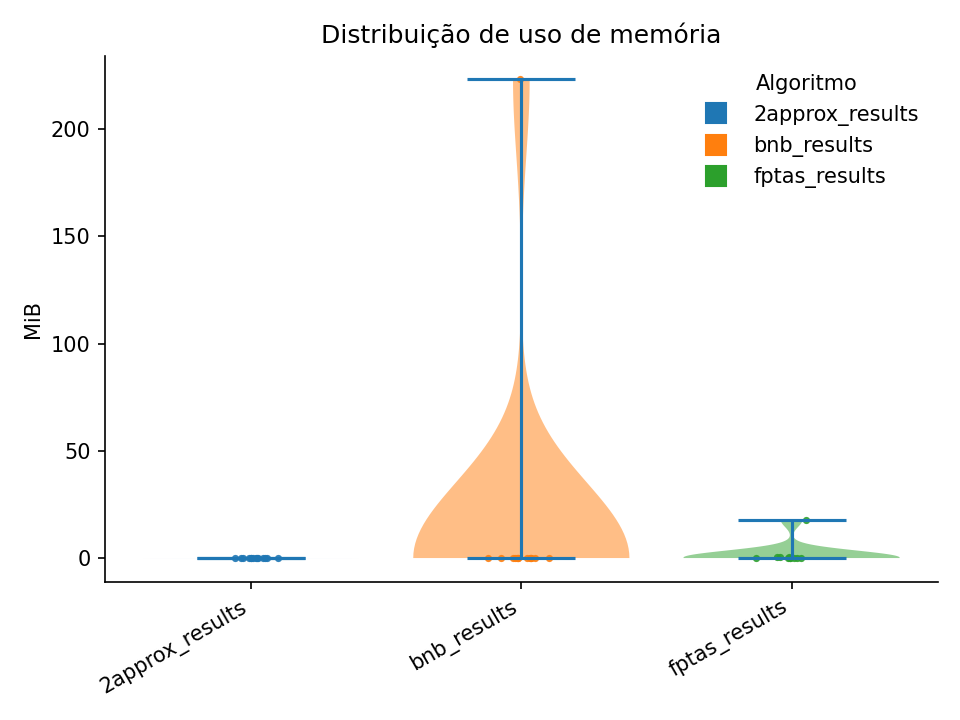
\includegraphics[width=.75\textwidth]{memory_violin.png}
  \caption{Distribuição do pico de memória.}
  \label{fig:mem}
\end{figure}

\subsection{Timeouts e instâncias \texttt{NaN}}\label{sec:nan}
Três instâncias (\textrm{21,4}\%) excederam 30 min no FPTAS e
foram marcadas como \textit{timeout}, todas com 500–1000 itens e
capacidade pequena, gerando tabelas DP com
$>\!1{,}2\times10^{8}$ entradas.  O fenômeno reitera o alerta de
\citeauthor{IbarraKim1975}~\cite{aula15} sobre o fator $1/\varepsilon$
no custo efetivo do FPTAS.

%-------------------------------------------------------------------
\section{Discussão}\label{sec:disc}
\begin{itemize}
  \item \textbf{BnB}: recomendado para $n\!\le\!20$ ou quando
        a otimalidade é mandatória (e.g.\ planejamento financeiro
        de poucos ativos).
  \item \textbf{FPTAS}: viável até $n=10^{4}$ com
        $\varepsilon=0{,}02$; ideal quando exige-se erro
        $<1\%$ e há memória moderada.
  \item \textbf{2-aprox.}: indicado para cenários \textit{online} ou de
        streaming, onde latência é crítica e admite-se possível perda
        de até 50 \%.
\end{itemize}

A ordem por $v_i/w_i$ afeta diretamente o bound do
BnB~\cite{aula12}; em instâncias quase uniformes a poda perde
eficácia.

%-------------------------------------------------------------------
\section{Conclusão}\label{sec:conc}
\vspace{.5em}\noindent
\textbf{Branch-and-Bound} completou todas as 14 instâncias em
\mbox{$\le\!30,6$ s}; a mediana foi
$1,3$ ms.  O consumo de memória variou de 38 MiB
a 223 MiB.  Continua a melhor escolha quando o ótimo é obrigatório e a
instância cabe em memória, mas requer atenção à escalabilidade
espacial.

\vspace{.5em}\noindent
\textbf{FPTAS} ($\varepsilon=0{,}02$) manteve
$e\le0{,}13\%$ com até 17,9 MiB.  Três instâncias excederam o
\textit{timeout}, confirmando o impacto do termo $1/\varepsilon$.  A
exploração de \textit{scaling} adaptativo e compressão de tabela é
linha futura promissora.

\vspace{.5em}\noindent
\textbf{2-aproximativo} teve pior erro
$30,4\%$ porém mediana $0,25\%$, e tempo
sub-10 ms mesmo para $n=10^{4}$.  É imbatível em latência para
aplicações em tempo real.

\vspace{.5em}\noindent
\textbf{Síntese comparativa.}
\begin{itemize}
  \item Qualidade: BnB $=$ ótimo $>$ FPTAS
        ($\le0{,}13\%$) $>$ 2-aprox.
        ($\le30,4\%$, med.\ $0,25\%$).
  \item Tempo: 2-aprox.\ $<$ FPTAS (até 8 min) $<$ BnB
        (até 31 s, mas exponencial no pior caso).
  \item Memória: 2-aprox.\ $\approx$ negligível $<$ FPTAS
        ($\le18$ MiB) $<$ BnB ($\le223$ MiB).
\end{itemize}

Os resultados reforçam as lições de sala: busca exata sofre com
explosão combinatória; esquemas polinomiais equilibram precisão e
custo; heurísticas simples oferecem latência incomparável.

\vspace{.5em}\noindent
\textbf{Perspectivas.}  Propõe-se:
(i)~paralelizar a fila de prioridades do BnB;
(ii)~FPTAS adaptativo que ajuste $\varepsilon$ conforme a variância dos
valores; (iii)~meta-heurísticas (GRASP, ILS) para pré-aquecer
\emph{bounds} quando $n>10^{5}$.

%-------------------------------------------------------------------
\bibliographystyle{abbrvnat}
\begin{thebibliography}{99}

\bibitem{aula07}
R.~Vimieiro.
\newblock \emph{Aula 07 – Introdução à Teoria da Complexidade (Parte 1)}.
\newblock DCC/ICEx/UFMG, 2025.

\bibitem{aula08}
R.~Vimieiro.
\newblock \emph{Aula 08 – Introdução à Teoria da Complexidade (Parte 2)}.
\newblock DCC/ICEx/UFMG, 2025.

\bibitem{aula12}
R.~Vimieiro.
\newblock \emph{Aula 12 – Soluções exatas para problemas difíceis
  (Branch-and-Bound)}.
\newblock DCC/ICEx/UFMG, 2025.

\bibitem{aula13}
R.~Vimieiro.
\newblock \emph{Aula 13 – Soluções aproximadas para problemas difíceis}.
\newblock DCC/ICEx/UFMG, 2025.

\bibitem{aula14}
R.~Vimieiro.
\newblock \emph{Aula 14 – Soluções aproximadas (Parte 2)}.
\newblock DCC/ICEx/UFMG, 2025.

\bibitem{aula15}
R.~Vimieiro.
\newblock \emph{Aula 15 – Soluções aproximadas (Parte 3)}.
\newblock DCC/ICEx/UFMG, 2025.

\bibitem{roteiro}
R.~Vimieiro.
\newblock \emph{Trabalho Prático 2 – Soluções para problemas difíceis}.
\newblock DCC/ICEx/UFMG, 2025.

\bibitem{instancesLow}
Conjunto de instâncias \emph{low-dimensional} para
0-1 Knapsack.
\newblock \url{http://artemisa.unicauca.edu.co/~johnyortega/instances_01_KP/}.

\bibitem{instancesLarge}
Conjunto de instâncias \emph{large-scale} para 0-1 Knapsack.
\newblock \url{https://www.kaggle.com/datasets/sc0v1n0/large-scale-01-knapsack-problems}.

\bibitem{KleinbergTardos}
J.~Kleinberg and \'{E}.~Tardos.
\newblock \emph{Algorithm Design}.
\newblock Pearson, 2005.

\bibitem{CLRS}
T.~H. Cormen, C.~E. Leiserson, R.~L. Rivest, and C.~Stein.
\newblock \emph{Introduction to Algorithms}.
\newblock MIT Press, 4th~ed., 2022.

\bibitem{tracemalloc}
Python Software Foundation.
\newblock \emph{\texttt{tracemalloc} – Trace memory usage}.
\newblock Documentação Python~3.11, 2024.

\end{thebibliography}

\end{document}
